\documentclass[a4paper]{article}
\usepackage{titling}
\usepackage{authblk}
\usepackage{fancyhdr}
\usepackage[hyphens]{url}
\usepackage{hyperref}
\usepackage{rsc}
\usepackage{siunitx}
\usepackage{graphicx}
\usepackage{mhchem}
\usepackage{amsmath}
\usepackage{listings}
\usepackage{color}
\usepackage[htt]{hyphenat}

\definecolor{dkgreen}{rgb}{0,0.6,0}
\definecolor{gray}{rgb}{0.5,0.5,0.5}
\definecolor{mauve}{rgb}{0.58,0,0.82}

\lstset{frame=tb,
  language=Python,
  aboveskip=3mm,
  belowskip=3mm,
  showstringspaces=false,
  columns=flexible,
  basicstyle={\ttfamily},
  numbers=none,
  numberstyle=\tiny\color{gray},
  keywordstyle=\color{blue},
  commentstyle=\color{dkgreen},
  stringstyle=\color{mauve},
  breaklines=true,
  breakatwhitespace=true,
  tabsize=3,
  postbreak=\mbox{\textcolor{red}{$\hookrightarrow$}\space}
}
\DeclareSIUnit\Fahrenheit{\degree F}

\title{Lecture 4: Debugging}
\author[1]{Dr Benjamin J. Morgan}
\author[1,2]{Dr Andrew R. McCluskey}
\affil[1]{Department of Chemistry, University of Bath, email: b.j.morgan@bath.ac.uk}
\affil[2]{Diamond Light Source, email: andrew.mccluskey@diamond.ac.uk}
\setcounter{Maxaffil}{0}
\renewcommand\Affilfont{\itshape\small}

\pagestyle{fancy}
\fancyhf{}
\rhead{CH40208}
\lhead{\thetitle}
\rfoot{\thepage}

\begin{document}
\maketitle

\section*{Aim}
This lecture will introduce \emph{debugging} skills and suggest methods to improve your ability to overcome errors in your code.

\section{Error messages}
Human beings are fallible, therefore code will have bugs.
However, there are some tips that we can use to deal with the bugs in our code and make them less of a nuesence.

One of the most powerful tools that is available to us is the quality of the code and libraries that are written in Python.
For example, if you \texttt{import} the square-root (\texttt{sqrt}) function from the basic Python library \texttt{math} and give it a list as an argument,
\begin{lstlisting}
from math import sqrt

a = [0, 1, 2, 3]

print(sqrt(a))
\end{lstlisting}
This will lead to an error.
However, this error will come with a \emph{traceback} showing where the error came from and will give some information, at the bottom, about why the error occurred.
You should get an error that looks like this,
\begin{lstlisting}
TypeError                                 Traceback (most recent call last)
<ipython-input-14-29539b5bdc2d> in <module>
----> 1 print(sqrt(a))

TypeError: must be real number, not list
\end{lstlisting}
As we can see, the error that has been thrown is a \texttt{TypeError}, and we are given the additional information about the error that: \texttt{must be real number, not list}.
We can use this to parse the root cause of the problem, a \texttt{TypeError} indicates that \emph{something} is of the wrong \emph{type}, and we are told that this \emph{something} should be a \texttt{real number} and not a \texttt{list}.
It is clear that the arugment being passed to the \texttt{sqrt()} function is of \emph{type} \texttt{list}, and therefore this is the problem.\footnote{Note that the \texttt{sqrt} function from the \texttt{math} library can only take single values and return the square-root. This NumPy \texttt{np.sqrt()} function can however handle objects of type \texttt{list} and NumPy arrays.}
\begin{table}[h]
	\centering
	\caption{Some error types that exist in Python.}
	\label{tab:ops}
	\begin{tabular}{c p{0.6\textwidth}}
		\hline
		Error & Context \\
		\hline
		\texttt{IndexError} & Trying to access an invalid index \\
		\texttt{ModuleNotFoundError} & Trying to import an non-existent module \\
		\texttt{TypeError} & Performing an action on an inappropriate type \\
		\texttt{ValueError} & Function argument is an inappropriate type \\
		\texttt{NameError} & Object with given variable name could not be found \\
		\texttt{ZeroDivisionError} & Trying to divide something by zero \\
		\hline
	\end{tabular}
\end{table}

\vspace{\baselineskip}
\begin{center}
	\noindent\fbox{%
	    \begin{minipage}{0.9\textwidth}%
	        \vspace{0.15\baselineskip}
			\subsubsection*{Exercise}
	        Try and determine the cause of the error messages thrown by the following commands (where a semi-colon indicated a new line):
          \begin{itemize}
            \item{\texttt{a = [0, 1, 2, 3]; np.square(a[-5])}}
            \item{\texttt{np.power(2)}}
            \item{\texttt{mp.array([1, 1, 2, 3, 5, 8, 13])}}
          \end{itemize}
          If you are not sure what a particular function does search for ``numpy'' and then the function name online, e.g. ``numpy power''.
	    \end{minipage}
	}
\end{center}

The majority of Python libraries will have helpful error messages such as the one given above (especially commonly used packages such as NumPy, pandas and matplotlib).
However, sometimes it is not immediately clear what the error message means, for this it is often necessary to leverage the most important tool in a programmers arsenal -- the internet.
Consider the following example, we have an array containing the numbers 1 to 9, which we reshape into a \texttt{(3, 3)} array and want to obtain the mean of each of the rows (where columns are the first axis and rows the second),
\begin{lstlisting}
import numpy as np

a = np.linspace(1, 9, 9)
a = np.reshape(a, (3, 3))

print(a)

print(np.mean(a, axis=2))
\end{lstlisting}
After running the above code, we will get the following error traceback,
\begin{lstlisting}
IndexError                                Traceback (most recent call last)
<ipython-input-16-d032bc661941> in <module>
----> 1 np.mean(a, axis=2)

~/python3.6/site-packages/numpy/core/fromnumeric.py in mean(a, axis, dtype, out, keepdims)
   3116
   3117     return _methods._mean(a, axis=axis, dtype=dtype,
-> 3118                           out=out, **kwargs)
   3119
   3120

~/python3.6/site-packages/numpy/core/_methods.py in _mean(a, axis, dtype, out, keepdims)
     60
     61     is_float16_result = False
---> 62     rcount = _count_reduce_items(arr, axis)
     63     # Make this warning show up first
     64     if rcount == 0:

~/python3.6/site-packages/numpy/core/_methods.py in _count_reduce_items(arr, axis)
     53     items = 1
     54     for ax in axis:
---> 55         items *= arr.shape[ax]
     56     return items
     57

IndexError: tuple index out of range
\end{lstlisting}
There is a lot of information here, but we want to focus on just the last line, which reads \texttt{IndexError: tuple index out of range}, which is rather opaque.
This is where the internet is our friend, if you \emph{copy and paste} this final line into Google\footnote{Or any decent search engine.}, you will likely find a lot of hits from a website called \textbf{Stack Overflow}.
Stack Overflow is a messageboard style website where people can post programming (and mathematics and general computation) questions and others will answer.
One of the great things about this website is that it is popular, so nearly all of the questions you could ask have already been answered.
%
\begin{figure}[t]
\centering
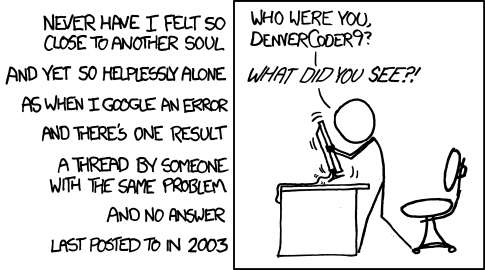
\includegraphics[width=0.8\textwidth]{wisdom_of_the_ancients}
\label{fig:wisdow}
\caption{Of course not every question will have an answer. Taken from xkcd (\url{https://xkcd.com/979/}).}
\end{figure}
%

If we put the error message from the above example into our search engine, we shoul be able to get some useful Stack Overflow answers.
For example\footnote{https://stackoverflow.com/questions/20296188/indexerror-tuple-index-out-of-range-python}, one of the answers suggests \emph{``I suspect you mean to say [0] where you say [1] and [1] where you say [2]. Indexes are 0-based in Python.''}, which can immediately lead us to our bug.
In the line \texttt{print(np.mean(a, axis=2))}, we assigned the row axis to the value $2$, however Python counts from $0$, to the column axis should be $0$, making the row axis $1$.
If we run the above code again with \texttt{axis=1}, we should get the following returned,
\begin{lstlisting}
[2. 5. 8.]
\end{lstlisting}
It may sound like a rather simple approach to debugging, however, the popularity of Python and the clarity of the error messages mean that \emph{Googling} the problem is often on of the quickest ways to debug a complex issue.

A final note on error messages is one of warning.
The nature of Python error messages are as \emph{tracebacks}, this means that the error traces back through the different levels of the library/code and then prints the cause of the error.
This means that Python error messages can be \textbf{very} long, take the code below (which makes use of the popular plotting library matplotlib) as an example,
\begin{lstlisting}
import numpy as np
import matplotlib.pyplot as plt

x = np.linspace(1, 10, 10)
y = np.linspace(1, 10, 9)

plt.plot(x, y)
plt.show()
\end{lstlisting}
Running this code will produce an error message that is more than 40 lines long and can be rather worrying the first time that you encounter it.
However, it is important not to worry about the size of the error message, but simply to scroll to the bottom of the page and to find the real reason for the error being thrown.
In the above example the error that is relevant is \texttt{ValueError: x and y must have same first dimension, but have shapes (10,) and (9,)}, which is relatively straight forward to parse.
One of the things we are plotting is an array of 10 numbers, while the other is an array of 9 (and therefore it doesn't make sense to plot them together).

\section{Overcoming problems}
The final component of this lecture is a brief (\emph{pseudo}-philosophical) discussion into how best to solve problems in programming.
It was mentioned above that one of the great things about using Python is the popularity of the language and the fact that this means that StackOverflow will very often have the answer to any problem you will encounter.
That statement comes with a caviat; the \emph{general} problem will probably be answered by someone previously, but your \emph{specific} problem will not have.

This is best represented with an example\footnote{This is a real example that I (Andrew) encountered while conducting research.}, where it is desired to rotate a chemical molecule in space by some given amount (the aim being to sample the system energy at a series of different rotations).
The first instinct when approaching this problem is to search for something like ``rotate molecule in space'', however, this gives a lot of information about rotational spectroscopy.
Adding ``stackoverflow'' at the end of that search starts to get us somewhere (\url{https://stackoverflow.com/questions/37942389/correctly-transforming-a-node-relative-to-a-specified-space}), however this is question is more advanced than what we are wanting to consider\footnote{This question is overly specific and the language used is not straight forward to understand.}.

However, if we detach the problem for the obvious chemical nature, it can be more general as a linear algebra, and indeed a fundemental aspect of computer visualisation.
For example, one of the top hits for the search of ``rotation 3d object'' is the wikipedia page for \emph{rotation matrices}, as usual the wikipedia page itself is too complex, but we may use this has a way to deepen our search.
Indeed, searching for ``rotation matrix chemical'' returns a LibreText page that discusses the mathematics of rotation matrices (\url{https://chem.libretexts.org/Bookshelves/Physical_and_Theoretical_Chemistry_Textbook_Maps/Book%3A_Symmetry_(Vallance)/09._Transformation_matrices}), and with continued searching you might end up at one of my favourite (and most useful papers) \cite{Evans2001}.

\section{Problem}
Using the work of Evans\cite{Evans2001}, write a function (and add it to your collection of functions for manipulating and quantifying chemical structures) that will rotate a diatomic molecule by a given set of Eulerian angles ($\alpha$, $\beta$, $\gamma$; see section 5.2 of the paper).
Calculate the distances between the two atoms of the molecule before and after the rotation to ensure that the this has not changed.
Test your code for a series of different rotations and atomic distances, and consider how the code that you have written might be relevant to applications in computational drug design.

\bibliographystyle{rsc}
\bibliography{handout_4}

\end{document}
